

\subsubsection{The layer editor}
To set up and edit the vertical device structure, use the layer editor this is shown in figure \ref{fig:layer_editor}. Using this tool, you can add layers, remove layers, and move layers up and down.
\linebreak
\linebreak 
\textbf{The first column}: This is a human readable name for the layer.
\linebreak 
\linebreak 
\textbf{The second column}: The thickness of the layer in meters.
\linebreak
\linebreak 
\textbf{Third column}: Sets the optical material properties.
\linebreak
\linebreak 
\textbf{Forth column}: Sets how the model treats the layer.  The optical equations are solved over all layers.  However, if the layer is set as 'active layer', then gpvdm will the also solve the electrical equations over this layer.  More than one layer can be set as an active layer, in this case, the electrical equations will be solved over all, the layers marked 'active layer', this is useful when simulating heterojunctions.  A layer type 'other', means that the electrical equations will not be solved over that layer, but the optical equations will be.  A layer type contact, denotes that the layer represents a contact layer.  This is only affects/is needed for 2/3D simulations.


\begin{figure}[ht!]
\centering
\includegraphics[width=\textwidth]{./images/layer_editor.png}
{\caption{The contact editor.}}
\label{fig:layer_editor}
\end{figure}

\subsubsection{The contact editor}

The contact editor is used to edit the contacts on the device, and what voltages are applied to which contacts, see figure \ref{fig:contact_editor}.  For a 1D simulation you can pretty much ignore this window.
\linebreak
\linebreak 
\textbf{The first column}: The human readable name for the contact.
\linebreak 
\linebreak 
\textbf{The second column}: Sets if the contact is at the top or bottom of the device.  There should be at least one contact at the top and one contact at the bottom of the device.  Some devices (OFETs) can have more than one contact at the top of the device. 
\linebreak
\linebreak 
\textbf{Third column}: This sets if the contact is 'active'.  In it's simplest form, an active contact is the contact to which the voltage ramp is applied during a JV curve simulation.  In a JV curve simulation, one contact will be held at 0 volts, while a steadily increasing voltage is applied to the other 'active' contact of the device.  If you are performing a transient voltage simulation, such as CELIV, the 'active' contact will have the CELIV voltage transient applied to it.  Swapping around the active contacts is equivalent to picking up the diode and turning it through 180 degrees and placing it back in the circuit.  This feature is most useful, when simulating OFETs, when one wants to apply a voltage ramp to one contact (i.e. the gate) out of three or four.
\linebreak
\linebreak 
\textbf{Forth column}: The start of the contact, not used in 1D simulations
\linebreak
\linebreak 
\textbf{Fifth column}: The width of the contact, not used in 1D simulations.
\linebreak
\linebreak
\textbf{Sixth column}: Sets the pasavation depth under the contact. Not used in 1D simulations.
\linebreak
\linebreak  
\textbf{Seventh column}: The sets the default voltage for a contact.  If the contact type is set as 'active', this value is ignored.  However, it the contact is not active, this voltage will appear on the contact.  This use useful in OFET simulations, where you want to hold a given contact at a set voltage. 
\linebreak
\linebreak  


\begin{figure}[ht!]
\centering
\includegraphics[width=\textwidth]{./images/contact_editor.png}
{\caption{The contact editor.}}
\label{fig:contact_editor}
\end{figure}



\subsubsection{Scanning parameters}
Sometimes one wishes to systematically vary a simulation parameter, this is how to do it:




\begin{figure}[ht!]
\centering
\includegraphics[width=\textwidth]{./images/1.jpg}
{\caption*{Step 1: Select the 'Parameter scan' tool.}}
\label{overflow}
\end{figure}


\begin{figure}[ht!]
\centering
\includegraphics[width=\textwidth]{./images/2.jpg}
\caption*{Step 2: Add a 'scan line' to the scan.}
\end{figure}

\begin{figure}[ht!]
\centering
\includegraphics[width=\textwidth]{./images/3.jpg}
\caption*{Step 3: Select the new 'scan line' and the click on the 'select parameter to change' tool.}
\label{overflow}
\end{figure}


\begin{figure}[ht!]
\centering
\includegraphics[width=\textwidth]{./images/4.jpg}
\caption*{Step 4: Select the parameter you want to change, click apply.}
\end{figure}


\begin{figure}[ht!]
\centering
\includegraphics[width=\textwidth]{./images/5.jpg}
\caption*{Step 5: The 'scan line' should now be updated with the parameter you want to scan.}
\end{figure}


\begin{figure}[ht!]
\centering
\includegraphics[width=\textwidth]{./images/6.jpg}
\caption*{Step 6: Now enter the parameters you wish to scan, in this case 0.0-0.5 suns.
Step 7: Click the run button.}
\end{figure}


\begin{figure}[ht!]
\centering
\includegraphics[width=\textwidth]{./images/7.jpg}
\caption*{Step 8: Select the output file you want to plot.  gpvdm will plot all simulation results.}
\end{figure}

\subsubsection{1D, 2D and 3D simulations with gpvdm}
When deciding if you should perform 1D, 2D or 3D, simulations, consider the dimensionality of your problem.  For example if you consider a solar cell, it is only a few micros thick, and there is rapid variation in the structure, charge densities, mobilities, and doping as a function of depth (y).  However, the structure will not vary very quickly in the lateral (xz) plane.  Therefore, in general  to capture all interesting effects present within a solar cell one only needs a 1D model.  If one now considers OFETs, there is both vertical an lateral current flow, therefore one can not get away with a 1D model any more, as one must simulate both vertical current flow, and current between the source and the drain, thus one needs a 2D simulation.  As the number of dimensions increases, computation speed will decrease, therefore my general advice is to use the minimum number of dimensions possible to solve your problem.

\subsubsection{Why don't I get a 3D view of the device}
If your simulation window looks like figure \ref{fig:nothreed} and not like figure \ref{fig:threed}.  It means  either you do not have any 3D acceleration hardware on your computer, or you do not have the drivers for it installed.  If you have an ATI/Nvidia/Intel graphics card check that the drivers are installed.  Currently, not having working 3D hardware will not affect your ability to perform simulations.

\begin{figure}[ht!]
\centering
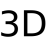
\includegraphics[width=\textwidth]{./images/3d.jpg}
\caption{gpvdm with working 3D acceleration hardware.}
\label{fig:threed}
\end{figure}

\begin{figure}[ht!]
\centering
\includegraphics[width=\textwidth]{./images/no_3d.jpg}
\caption{gpvdm with no 3D acceleration hardware.}
\label{fig:nothreed}
\end{figure}

\vfill
\clearpage


\newpage




\section{The user interface}
\subsubsection{Is Langevin recombination a good way of describing recombination OPV devices?}
In my view Langevin recombination is in general a really bad way to describe recombination in OPV devices.  This is because the mechanism assumes Brownian motion of electrons and holes and that charge carriers of opposite polarity will recombine when they get close enough to fall into each others electrostatic field.  This picture assumes the charge carriers are free and completely neglects the influence of trap states.  I therefore think Langeving recombination should be avoided in OPVs.
But in dx.doi.org/10.1021/jp200234m you used Langevin recombination - why?: In this paper I allowed the mobility in the Langevin expression to vary as a function of carrier density i.e.
\begin{equation}
R_{free}=q k_{r}\frac{(\alpha \mu_e(n)+\beta \mu_h(n)) n_{tot} p_{tot}}{2\epsilon_0\epsilon_r}
\end{equation}

I then by defining a mobility edge and assuming any carrier below the mobility edge could not move and any carrier above it could.  I could define the averaged electron/hole mobility as: 

\begin{equation}
\mu_e(n)=\frac{\mu_e^0 n_{free}}{n_{free}+n_{trap}}
\end{equation}

and

\begin{equation}
\mu_h(n)=\frac{\mu_h^0 p_{free}}{p_{free}+p_{trap}}
\end{equation}

and if one assumes the density of free charge carriers is much smaller than the density of trapped charge carriers one can arrive at

\begin{equation}
R(n,p)=q k_{r}\frac{(\alpha \mu_e^0 n_{free} p_{trap}+\beta \mu_h p_{free} n_{trap}) }{2\epsilon_0\epsilon_r}
\end{equation}

Thus by making the mobility carrier density dependent we arrive at an expression for Langeving recombination that's dependent upon the density of free and trapped carriers (i.e. $n_{free} p_{trap}$ and $ p_{free} n_{trap}$) This is in principle the same as SRH recombination (i.e. a process involving free electrons (holes) recombining with trapped holes (electrons)).  This was a nice simple approach and it worked quite well in the steady state.  However, to make this all work I had to assume all electrons (holes) at any given position in space had a single quasi-Fermi level, which meant they were all in equilibrium with each other.  For this to be true, all electrons (holes) would have to be able to exchange energy with all other electrons (holes) at that position in space and have an infinite charge carrier thermalization velocity.  This seemed like an OK assumption in steady state when electrons (holes) had time to exchange energy, however once we start thinking about things happening in time domain, it becomes harder to justify because there are so many trap states in the device it is unlikely that charge carriers will be able to act as one equilibrated gas with one quasi-Fermi level.  On the other hand the SRH mechanism does not make this assumption, so it is probably a better description of recombination/trapping.  I would also add that I have never found a situation in OPV device modeling where SRH recombination was unable to describe the device in question.  Conclusion: SRH is better than Langevin.  


\subsubsection{Should I trust the results of gpvdm?}
Yes!  The model it's self has been verified against experiment [there are over 20 publications doing this, in steady state, time domain (us-fs time scales), and fx-domain]. The basic drift-diffusion solver was cross checked and compared against other drift diffusion models, and the accuracy compared down to 6-9 dp.  While the optical model has been compared to analytical solutions of Maxwell's equations.  The SRH model has also been compared against analytical models.  If the answers you are getting out of gpvdm are odd, then I would suggest to take a look at the input parameters.  If your efficienceis are high, try increasing the number of trap states, the recombination cross sections or reducing the e/h mobilites.  Finally, I would also recommend always running the latest version, and keeping an eye on the twitter stream for bug announcements.



\subsection{Can I use the model to simulate my exotic* material system/contacts?}
The short answer is yes.  The model is an effective medium model, meaning that it does not simulate the details of the medium, rather it approximates the medium with a set of electrical parameters.  For example, when simulating an organic solar cell, it does not simulate every detail of the BHJ, rather it just assumes an effective mobility, density of states, recombination cross sections, trapping cross sections and so on...  So if you can find electrical parameters to aproximate your material system (or guess them), there is nothing stopping you using gpvdm to simulate any exotic device/material.  The same goes for the contacts, the model simulates the contacts simply as a charge density. So if you have fancy graphene contacts which inject lots of charge, use a high majority carrier density on the contacts.  Where as if you have some dirty old ITO contacts may be drop the majority carrier density a bit.

\newpage


\section{Output directories}
\textbf{equilibrium}\newline
Before the solver starts any simulation it solves the device equations in the dark with 0V applied bias.  The result of this calculation are placed in this directory.  The practical reason for doing this is that Newton's method only works if you give it a reasonable starting guess for any given problem.  Thus to start the solver, we guess the carrier densities at 0V in the dark, we then use Newton's method to calculate the exact carrier density profiles at 0V in the dark (results are stored in the equilibrium directory), then from this point we can work our way to other solutions say at +1V in the light.\cite{0953-8984-25-21-215301}
\newline

\section{Output files}
Writing to disk is slow on even the most modern of computers with an SSD.  The seek speed of mechanical disks has increased little of their history.  Thus often writing the output data to the hard disk is the most time consuming part of any simulation.  By default gpvdm writes all output files to disk.  If you want to speed up your simulation, you can only write the files you need to disk.  This can be done in a fine grained way through the configure window and clicking on the detailed dump control tab.  You will from there be able to turn on and off output files.

\begin{figure}
\centering
\includegraphics[width=\textwidth]{./images/output_files.png}
\caption{Selecting which output files are witten to disk.}
\end{figure}

\subsubsection{1D position space output}
\paragraph{Band structure}
\textbf{Ec.dat}:LUMO-position\newline
x-axis:Position($nm$)\newline
y-axis:Electron Energy($eV$)\newline
\newline
\textbf{Efield.dat}:Material number - position\newline
x-axis:Position($nm$)\newline
y-axis:Number($au$)\newline
\newline
\textbf{Eg.dat}:Band gap-position\newline
x-axis:Position($nm$)\newline
y-axis:Electron Energy($eV$)\newline
\newline
\textbf{Ev.dat}:HOMO-position\newline
x-axis:Position($nm$)\newline
y-axis:Electron Energy($eV$)\newline
\newline
\textbf{Fi.dat}:Equlibrium Fermi-level - position\newline
x-axis:Position($nm$)\newline
y-axis:Energy($eV$)\newline
\newline
\textbf{Fn.dat}:Electron quasi Fermi-level position\newline
x-axis:Position($nm$)\newline
y-axis:Electron Energy($eV$)\newline
\newline
\textbf{Fp.dat}:Hole quasi Fermi-level position\newline
x-axis:Position($nm$)\newline
y-axis:Electron Energy($eV$)\newline
\newline
\textbf{phi.dat}:Potential\newline
x-axis:Position($nm$)\newline
y-axis:Potential($V$)\newline
\newline
\paragraph{Chaerge density}
\textbf{dn.dat}:Change in free electron population - position\newline
x-axis:Position($nm$)\newline
y-axis:Carrier density($m^{-3}$)\newline
\newline
\paragraph{Charge density}
\textbf{Nad.dat}:Doping - position\newline
x-axis:Position($nm$)\newline
y-axis:Doping density($m^{-3}$)\newline
\newline
\textbf{dnt.dat}:Excess electron density - position\newline
x-axis:Position($nm$)\newline
y-axis:Electron density($m^{-3}$)\newline
\newline
\textbf{dp.dat}:Change in free hole population - position\newline
x-axis:Position($nm$)\newline
y-axis:Carrier density($m^{-3}$)\newline
\newline
\textbf{dpt.dat}:Excess electron density - position\newline
x-axis:Position($nm$)\newline
y-axis:Hole density($m^{-3}$)\newline
\newline
\textbf{n.dat}:Total hole density - position\newline
x-axis:Position($nm$)\newline
y-axis:Carrier density($m^{-3}$)\newline
\newline
\textbf{nt.dat}:Trapped electron carrier density - position\newline
x-axis:Position($nm$)\newline
y-axis:Carrier density($m^{-3}$)\newline
\newline
\textbf{p.dat}:Total hole density - position\newline
x-axis:Position($nm$)\newline
y-axis:Carrier density($m^{-3}$)\newline
\newline
\textbf{pt.dat}:Trapped hole carrier density - position\newline
x-axis:Position($nm$)\newline
y-axis:Carrier density($m^{-3}$)\newline
\newline
\paragraph{Material parameters}
\textbf{epsilon\_r.dat}:Relative permittivity - position\newline
x-axis:Position($nm$)\newline
y-axis:Relative permittivity($au$)\newline
\newline
\textbf{mu\_n.dat}:Electron mobility - position\newline
x-axis:Position($nm$)\newline
y-axis:Electron mobility($m^{2} V^{-1} s^{-1}$)\newline
\newline
\textbf{mu\_n\_ft.dat}:Electron mobility free/all- position\newline
x-axis:Position($nm$)\newline
y-axis:Mobility($m^{2} V^{-1} s^{-1}$)\newline
\newline
\textbf{mu\_p.dat}:Hole mobility - position\newline
x-axis:Position($nm$)\newline
y-axis:Hole mobility($m^{2} V^{-1} s^{-1}$)\newline
\newline
\textbf{mu\_p\_ft.dat}:Hole mobility free/all- position\newline
x-axis:Position($nm$)\newline
y-axis:Mobility($m^{2} V^{-1} s^{-1}$)\newline
\newline
\textbf{nf.dat}:Free electron carrier density - position\newline
x-axis:Position($nm$)\newline
y-axis:Carrier density($m^{-3}$)\newline
\newline
\textbf{pf.dat}:Free hole carrier density - position\newline
x-axis:Position($nm$)\newline
y-axis:Carrier density($m^{-3}$)\newline
\newline
\paragraph{Model}
\textbf{imat.dat}:Material number - position\newline
x-axis:Position($nm$)\newline
y-axis:Number($au$)\newline
\newline
\paragraph{Recombination}
\textbf{Gn.dat}:Free electron generation rate - position\newline
x-axis:Position($nm$)\newline
y-axis:Generation rate($m^{-3} s^{-1}$)\newline
\newline
\textbf{Gp.dat}:Free hole generation rate - position\newline
x-axis:Position($nm$)\newline
y-axis:Generation rate($m^{-3} s^{-1}$)\newline
\newline
\textbf{Rn\_srh.dat}:SRH electron recombination rate - position\newline
x-axis:Position($nm$)\newline
y-axis:Recombination rate($m^{-3} s^{-1}$)\newline
\newline
\textbf{Rp\_srh.dat}:SRH hole recombination rate - position\newline
x-axis:Position($nm$)\newline
y-axis:Recombination rate($m^{-3} s^{-1}$)\newline
\newline
\textbf{R\_free.dat}:Free electron-hole recombination rate - position\newline
x-axis:Position($nm$)\newline
y-axis:Recombination rate($m^{-3} s^{-1}$)\newline
\newline
\textbf{fsrhh.dat}:Trap fermi level - position\newline
x-axis:Position($nm$)\newline
y-axis:Electron Fermi level($eV$)\newline
\newline
\textbf{fsrhn.dat}:Trap fermi level - position\newline
x-axis:Position($nm$)\newline
y-axis:Electron Fermi level($eV$)\newline
\newline
\textbf{nf\_to\_pt.dat}:Free electron to trapped hole - position\newline
x-axis:Position($nm$)\newline
y-axis:Rate($m^{-3} s^{-1}$)\newline
\newline
\textbf{nrelax.dat}:Electron relaxation rate - position\newline
x-axis:Position($nm$)\newline
y-axis:Rate($m^{-3} s^{-1}$)\newline
\newline
\textbf{pf\_to\_nt.dat}:Free hole to trapped electron - position\newline
x-axis:Position($nm$)\newline
y-axis:Rate($m^{-3} s^{-1}$)\newline
\newline
\textbf{prelax.dat}:Hole relaxation rate - position\newline
x-axis:Position($nm$)\newline
y-axis:Rate($m^{-3} s^{-1}$)\newline
\newline

\textbf{Photon\_gen.dat}:Photon generation rate - position\newline
x-axis:Position($nm$)\newline
y-axis:Photon generation rate($m^{-3} s^{-1}$)\newline

\paragraph{Transport}
\textbf{Jn.dat}:Current density - position\newline
x-axis:Position($nm$)\newline
y-axis:Electron current density($A m^{-2}$)\newline
\newline
\textbf{Jn\_diffusion.dat}:Diffusion current density - position\newline
x-axis:Position($nm$)\newline
y-axis:Electron current density (diffusion)($A m^{-2}$)\newline
\newline
\textbf{Jn\_drift.dat}:Drift current density - position\newline
x-axis:Position($nm$)\newline
y-axis:Electron current density (drift)($A m^{-2}$)\newline
\newline
\textbf{Jn\_plus\_Jp.dat}:Total current density (Jn+Jp) - position\newline
x-axis:Position($nm$)\newline
y-axis:Total current density (Jn+Jp)($A m^{-2}$)\newline
\newline
\textbf{Jp.dat}:Current density - position\newline
x-axis:Position($nm$)\newline
y-axis:Hole current density($A m^{-2}$)\newline
\newline
\textbf{Jp\_diffusion.dat}:Diffusion current density - position\newline
x-axis:Position($nm$)\newline
y-axis:Hole current density (diffusion)($A m^{-2}$)\newline
\newline
\textbf{Jp\_drift.dat}:Drift current density - position\newline
x-axis:Position($nm$)\newline
y-axis:Hole current density (drift)($A m^{-2}$)\newline
\newline
\textbf{Jp\_drift\_plus\_diffusion.dat}:Total current density (Jn+Jp) - position\newline
x-axis:Position($nm$)\newline
y-axis:Total current density (Jn+Jp)($A m^{-2}$)\newline
\newline


\textbf{sim\_info.dat}\newline
This file contains quantities calculated from the simulation such as $V_{oc}$, $J_{sc}$ what is in the file depends on what type of simulation you whish to carry out.  The file is a JSON formatted file file some common tokens are defined below:

JV curve simulation:

\begin{center}
\begin{tabular}{ |c|c|c| c|} 
\hline
JSON token & Meaning & Units & Ref \\
\hline
ff & Fill factor&au&\\
pce & 			PCE& percent&\\
Pmax & 			Power at Pmax&&\\
voc & 			$V_{oc}$ &&\\
$voc_{R}$ & 		Recombination rate at $P_{max}$& &\\
$jv_{voc}$  & 		&&\\
$jv_{pmax}$ & 	&&\\
$voc_{nt}$ & Trapped electron carrier densiyt at $V_oc$		&&\\
$voc_{pt}$ & Trapped hole carrier density at $V_oc$		&&\\
$voc_{nf}$ & Free electron carrier densiyt at $V_oc$		&&\\
$voc_{pf}$ & Free hole carrier density at $V_oc$		&&\\
jsc 				  & 	$J_{sc}$		& $Am^{-2}$&\\
$jv_{jsc}$ & Average charge density at $J_{sc}$	& $m^{-3}$&\\
$jv_{vbi}$ & Built in voltage		& V&\\
$jv_{gen}$ & Average generation rate		&&\\
$voc_{np}$ & 	&&\\
$j_{pmax}$ & Current at $P_{max}$		& $Am^{-2}$&\\
$v_{pmax}$ & Voltage at $P_{max}$    & V &\\
$mu_{jsc}$ & 		&$m^{2} V^{-1} s^{-1}$&\\
$mu_{pmax}$ & 		&$m^{2} V^{-1} s^{-1}$&\\
$mu_{voc}$ & 	Average mobility at $V_{oc}$	& $m^{2} V^{-1} s^{-1}$&\\
$mue_{pmax}$ & Average electron mobility at $P_{max}$	&$m^{2} V^{-1} s^{-1}$&\\
$muh_{pmax}$ & Average hole mobility at $P_{max}$ &$m^{2} V^{-1} s^{-1}$&\\
$tau_{voc}$ & 	Recombination time constant at $V_{oc}$	 & s &\\
$tau_{pmax}$ & 	Recombination time constant at $P_{max}$	&s&\\

$theta_{srh}$ & $\theta_{SRH}$ Collection coefficient at $P_{max}$ y & au &p.100 5.2a\cite{Summon-FETCH-bonn_catalog_45326403},\cite{PhysRevApplied.6.024001}\\
$theta_{srh}$ & $\theta_{SRH}$ Collection coefficient at $P_{max}$ & au &p.100 5.2a\cite{Summon-FETCH-bonn_catalog_45326403},\cite{PhysRevApplied.6.024001}\\

\hline
\end{tabular}
\end{center}

Optical simulation

\begin{center}
\begin{tabular}{ |c|c|c| c|} 
\hline
JSON token & Meaning & Units & Ref \\
\hline
$J_{photo}$ & Photo current density $Am^{-2}$& &\\
$I_{photo}$ & Photo current $A$& &\\


\hline
\end{tabular}
\end{center}

\section{Copyright of the manual}
This manual is released under CC-BY license.

